% Created by tikzDevice version 0.6.2-92-0ad2792 on 2013-02-14 02:54:48
% !TEX encoding = UTF-8 Unicode
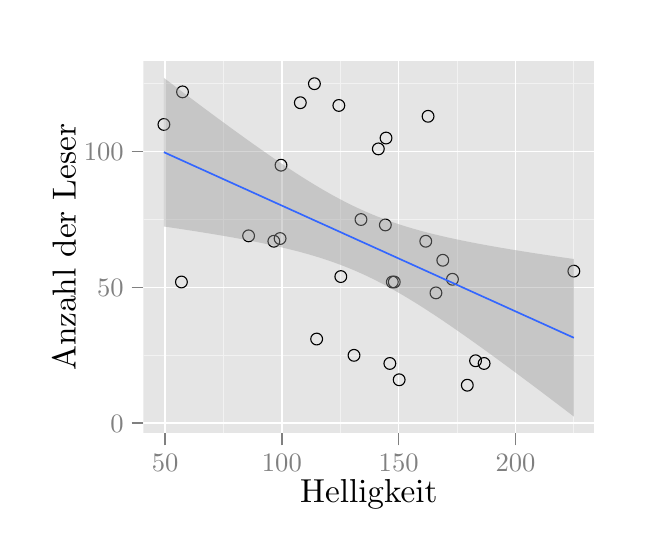
\begin{tikzpicture}[x=1pt,y=1pt]
\definecolor[named]{fillColor}{rgb}{1.00,1.00,1.00}
\path[use as bounding box,fill=fillColor,fill opacity=0.00] (0,0) rectangle (216.81,180.67);
\begin{scope}
\path[clip] (  0.00,  0.00) rectangle (216.81,180.67);
\definecolor[named]{drawColor}{rgb}{1.00,1.00,1.00}
\definecolor[named]{fillColor}{rgb}{1.00,1.00,1.00}

\path[draw=drawColor,line width= 0.6pt,line join=round,line cap=round,fill=fillColor] (  0.00,  0.00) rectangle (216.81,180.68);
\end{scope}
\begin{scope}
\path[clip] ( 41.82, 34.03) rectangle (204.77,168.63);
\definecolor[named]{fillColor}{rgb}{0.90,0.90,0.90}

\path[fill=fillColor] ( 41.82, 34.03) rectangle (204.77,168.63);
\definecolor[named]{drawColor}{rgb}{0.95,0.95,0.95}

\path[draw=drawColor,line width= 0.3pt,line join=round] ( 41.82, 62.27) --
	(204.77, 62.27);

\path[draw=drawColor,line width= 0.3pt,line join=round] ( 41.82,111.34) --
	(204.77,111.34);

\path[draw=drawColor,line width= 0.3pt,line join=round] ( 41.82,160.42) --
	(204.77,160.42);

\path[draw=drawColor,line width= 0.3pt,line join=round] ( 70.75, 34.03) --
	( 70.75,168.63);

\path[draw=drawColor,line width= 0.3pt,line join=round] (112.95, 34.03) --
	(112.95,168.63);

\path[draw=drawColor,line width= 0.3pt,line join=round] (155.15, 34.03) --
	(155.15,168.63);

\path[draw=drawColor,line width= 0.3pt,line join=round] (197.35, 34.03) --
	(197.35,168.63);
\definecolor[named]{drawColor}{rgb}{1.00,1.00,1.00}

\path[draw=drawColor,line width= 0.6pt,line join=round] ( 41.82, 37.73) --
	(204.77, 37.73);

\path[draw=drawColor,line width= 0.6pt,line join=round] ( 41.82, 86.81) --
	(204.77, 86.81);

\path[draw=drawColor,line width= 0.6pt,line join=round] ( 41.82,135.88) --
	(204.77,135.88);

\path[draw=drawColor,line width= 0.6pt,line join=round] ( 49.65, 34.03) --
	( 49.65,168.63);

\path[draw=drawColor,line width= 0.6pt,line join=round] ( 91.85, 34.03) --
	( 91.85,168.63);

\path[draw=drawColor,line width= 0.6pt,line join=round] (134.05, 34.03) --
	(134.05,168.63);

\path[draw=drawColor,line width= 0.6pt,line join=round] (176.25, 34.03) --
	(176.25,168.63);
\definecolor[named]{drawColor}{rgb}{0.00,0.00,0.00}

\path[draw=drawColor,line width= 0.4pt,line join=round,line cap=round] (113.15, 90.73) circle (  2.13);

\path[draw=drawColor,line width= 0.4pt,line join=round,line cap=round] (197.36, 92.70) circle (  2.13);

\path[draw=drawColor,line width= 0.4pt,line join=round,line cap=round] ( 91.54,130.97) circle (  2.13);

\path[draw=drawColor,line width= 0.4pt,line join=round,line cap=round] (161.84, 60.31) circle (  2.13);

\path[draw=drawColor,line width= 0.4pt,line join=round,line cap=round] (158.86, 51.47) circle (  2.13);

\path[draw=drawColor,line width= 0.4pt,line join=round,line cap=round] (104.42, 68.16) circle (  2.13);

\path[draw=drawColor,line width= 0.4pt,line join=round,line cap=round] (126.71,136.86) circle (  2.13);

\path[draw=drawColor,line width= 0.4pt,line join=round,line cap=round] (131.77, 88.77) circle (  2.13);

\path[draw=drawColor,line width= 0.4pt,line join=round,line cap=round] (153.50, 89.75) circle (  2.13);

\path[draw=drawColor,line width= 0.4pt,line join=round,line cap=round] (132.47, 88.77) circle (  2.13);

\path[draw=drawColor,line width= 0.4pt,line join=round,line cap=round] (130.87, 59.33) circle (  2.13);

\path[draw=drawColor,line width= 0.4pt,line join=round,line cap=round] (147.53, 84.84) circle (  2.13);

\path[draw=drawColor,line width= 0.4pt,line join=round,line cap=round] ( 91.21,104.47) circle (  2.13);

\path[draw=drawColor,line width= 0.4pt,line join=round,line cap=round] (144.68,148.64) circle (  2.13);

\path[draw=drawColor,line width= 0.4pt,line join=round,line cap=round] (164.93, 59.33) circle (  2.13);

\path[draw=drawColor,line width= 0.4pt,line join=round,line cap=round] (129.24,109.38) circle (  2.13);

\path[draw=drawColor,line width= 0.4pt,line join=round,line cap=round] (120.44,111.34) circle (  2.13);

\path[draw=drawColor,line width= 0.4pt,line join=round,line cap=round] ( 49.23,145.69) circle (  2.13);

\path[draw=drawColor,line width= 0.4pt,line join=round,line cap=round] (143.85,103.49) circle (  2.13);

\path[draw=drawColor,line width= 0.4pt,line join=round,line cap=round] (150.00, 96.62) circle (  2.13);

\path[draw=drawColor,line width= 0.4pt,line join=round,line cap=round] (134.24, 53.44) circle (  2.13);

\path[draw=drawColor,line width= 0.4pt,line join=round,line cap=round] ( 98.52,153.55) circle (  2.13);

\path[draw=drawColor,line width= 0.4pt,line join=round,line cap=round] ( 79.83,105.45) circle (  2.13);

\path[draw=drawColor,line width= 0.4pt,line join=round,line cap=round] ( 88.95,103.49) circle (  2.13);

\path[draw=drawColor,line width= 0.4pt,line join=round,line cap=round] (103.61,160.42) circle (  2.13);

\path[draw=drawColor,line width= 0.4pt,line join=round,line cap=round] ( 55.95,157.47) circle (  2.13);

\path[draw=drawColor,line width= 0.4pt,line join=round,line cap=round] (112.44,152.56) circle (  2.13);

\path[draw=drawColor,line width= 0.4pt,line join=round,line cap=round] (117.92, 62.27) circle (  2.13);

\path[draw=drawColor,line width= 0.4pt,line join=round,line cap=round] ( 55.56, 88.77) circle (  2.13);

\path[draw=drawColor,line width= 0.4pt,line join=round,line cap=round] (129.49,140.79) circle (  2.13);
\definecolor[named]{fillColor}{rgb}{0.60,0.60,0.60}

\path[fill=fillColor,fill opacity=0.40] ( 49.23,162.51) --
	( 51.10,161.09) --
	( 52.98,159.67) --
	( 54.85,158.26) --
	( 56.73,156.84) --
	( 58.60,155.43) --
	( 60.48,154.03) --
	( 62.35,152.63) --
	( 64.23,151.23) --
	( 66.10,149.84) --
	( 67.98,148.45) --
	( 69.85,147.07) --
	( 71.73,145.70) --
	( 73.60,144.33) --
	( 75.48,142.97) --
	( 77.35,141.62) --
	( 79.23,140.27) --
	( 81.10,138.93) --
	( 82.98,137.61) --
	( 84.85,136.29) --
	( 86.73,134.99) --
	( 88.60,133.69) --
	( 90.48,132.42) --
	( 92.35,131.15) --
	( 94.23,129.90) --
	( 96.10,128.67) --
	( 97.98,127.46) --
	( 99.85,126.27) --
	(101.73,125.10) --
	(103.60,123.95) --
	(105.48,122.83) --
	(107.35,121.74) --
	(109.23,120.67) --
	(111.10,119.63) --
	(112.98,118.63) --
	(114.85,117.65) --
	(116.73,116.71) --
	(118.60,115.81) --
	(120.48,114.94) --
	(122.35,114.11) --
	(124.23,113.31) --
	(126.10,112.54) --
	(127.98,111.81) --
	(129.86,111.11) --
	(131.73,110.44) --
	(133.61,109.81) --
	(135.48,109.20) --
	(137.36,108.62) --
	(139.23,108.06) --
	(141.11,107.53) --
	(142.98,107.02) --
	(144.86,106.53) --
	(146.73,106.06) --
	(148.61,105.61) --
	(150.48,105.17) --
	(152.36,104.75) --
	(154.23,104.34) --
	(156.11,103.95) --
	(157.98,103.56) --
	(159.86,103.19) --
	(161.73,102.83) --
	(163.61,102.47) --
	(165.48,102.13) --
	(167.36,101.79) --
	(169.23,101.46) --
	(171.11,101.13) --
	(172.98,100.82) --
	(174.86,100.50) --
	(176.73,100.20) --
	(178.61, 99.89) --
	(180.48, 99.60) --
	(182.36, 99.30) --
	(184.23, 99.01) --
	(186.11, 98.73) --
	(187.98, 98.45) --
	(189.86, 98.17) --
	(191.73, 97.89) --
	(193.61, 97.62) --
	(195.48, 97.35) --
	(197.36, 97.08) --
	(197.36, 40.15) --
	(195.48, 41.58) --
	(193.61, 43.01) --
	(191.73, 44.43) --
	(189.86, 45.85) --
	(187.98, 47.27) --
	(186.11, 48.69) --
	(184.23, 50.10) --
	(182.36, 51.51) --
	(180.48, 52.91) --
	(178.61, 54.31) --
	(176.73, 55.71) --
	(174.86, 57.10) --
	(172.98, 58.48) --
	(171.11, 59.86) --
	(169.23, 61.24) --
	(167.36, 62.60) --
	(165.48, 63.96) --
	(163.61, 65.31) --
	(161.73, 66.66) --
	(159.86, 67.99) --
	(157.98, 69.32) --
	(156.11, 70.63) --
	(154.23, 71.93) --
	(152.36, 73.22) --
	(150.48, 74.50) --
	(148.61, 75.76) --
	(146.73, 77.00) --
	(144.86, 78.23) --
	(142.98, 79.44) --
	(141.11, 80.63) --
	(139.23, 81.79) --
	(137.36, 82.93) --
	(135.48, 84.05) --
	(133.61, 85.14) --
	(131.73, 86.20) --
	(129.86, 87.23) --
	(127.98, 88.23) --
	(126.10, 89.20) --
	(124.23, 90.13) --
	(122.35, 91.03) --
	(120.48, 91.89) --
	(118.60, 92.72) --
	(116.73, 93.51) --
	(114.85, 94.27) --
	(112.98, 94.99) --
	(111.10, 95.68) --
	(109.23, 96.34) --
	(107.35, 96.98) --
	(105.48, 97.58) --
	(103.60, 98.15) --
	(101.73, 98.70) --
	( 99.85, 99.23) --
	( 97.98, 99.74) --
	( 96.10,100.22) --
	( 94.23,100.69) --
	( 92.35,101.14) --
	( 90.48,101.57) --
	( 88.60,101.99) --
	( 86.73,102.40) --
	( 84.85,102.79) --
	( 82.98,103.17) --
	( 81.10,103.54) --
	( 79.23,103.90) --
	( 77.35,104.26) --
	( 75.48,104.60) --
	( 73.60,104.94) --
	( 71.73,105.27) --
	( 69.85,105.59) --
	( 67.98,105.91) --
	( 66.10,106.22) --
	( 64.23,106.52) --
	( 62.35,106.82) --
	( 60.48,107.12) --
	( 58.60,107.41) --
	( 56.73,107.70) --
	( 54.85,107.99) --
	( 52.98,108.27) --
	( 51.10,108.55) --
	( 49.23,108.82) --
	cycle;
\definecolor[named]{drawColor}{rgb}{0.20,0.40,1.00}

\path[draw=drawColor,line width= 0.6pt,line join=round] ( 49.23,135.67) --
	( 51.10,134.82) --
	( 52.98,133.97) --
	( 54.85,133.12) --
	( 56.73,132.27) --
	( 58.60,131.42) --
	( 60.48,130.57) --
	( 62.35,129.73) --
	( 64.23,128.88) --
	( 66.10,128.03) --
	( 67.98,127.18) --
	( 69.85,126.33) --
	( 71.73,125.48) --
	( 73.60,124.63) --
	( 75.48,123.78) --
	( 77.35,122.94) --
	( 79.23,122.09) --
	( 81.10,121.24) --
	( 82.98,120.39) --
	( 84.85,119.54) --
	( 86.73,118.69) --
	( 88.60,117.84) --
	( 90.48,116.99) --
	( 92.35,116.15) --
	( 94.23,115.30) --
	( 96.10,114.45) --
	( 97.98,113.60) --
	( 99.85,112.75) --
	(101.73,111.90) --
	(103.60,111.05) --
	(105.48,110.20) --
	(107.35,109.36) --
	(109.23,108.51) --
	(111.10,107.66) --
	(112.98,106.81) --
	(114.85,105.96) --
	(116.73,105.11) --
	(118.60,104.26) --
	(120.48,103.41) --
	(122.35,102.57) --
	(124.23,101.72) --
	(126.10,100.87) --
	(127.98,100.02) --
	(129.86, 99.17) --
	(131.73, 98.32) --
	(133.61, 97.47) --
	(135.48, 96.62) --
	(137.36, 95.78) --
	(139.23, 94.93) --
	(141.11, 94.08) --
	(142.98, 93.23) --
	(144.86, 92.38) --
	(146.73, 91.53) --
	(148.61, 90.68) --
	(150.48, 89.83) --
	(152.36, 88.99) --
	(154.23, 88.14) --
	(156.11, 87.29) --
	(157.98, 86.44) --
	(159.86, 85.59) --
	(161.73, 84.74) --
	(163.61, 83.89) --
	(165.48, 83.04) --
	(167.36, 82.20) --
	(169.23, 81.35) --
	(171.11, 80.50) --
	(172.98, 79.65) --
	(174.86, 78.80) --
	(176.73, 77.95) --
	(178.61, 77.10) --
	(180.48, 76.25) --
	(182.36, 75.41) --
	(184.23, 74.56) --
	(186.11, 73.71) --
	(187.98, 72.86) --
	(189.86, 72.01) --
	(191.73, 71.16) --
	(193.61, 70.31) --
	(195.48, 69.46) --
	(197.36, 68.62);
\end{scope}
\begin{scope}
\path[clip] (  0.00,  0.00) rectangle (216.81,180.67);
\definecolor[named]{drawColor}{rgb}{0.50,0.50,0.50}

\node[text=drawColor,anchor=base east,inner sep=0pt, outer sep=0pt, scale=  0.96] at ( 34.71, 34.43) {0};

\node[text=drawColor,anchor=base east,inner sep=0pt, outer sep=0pt, scale=  0.96] at ( 34.71, 83.50) {50};

\node[text=drawColor,anchor=base east,inner sep=0pt, outer sep=0pt, scale=  0.96] at ( 34.71,132.57) {100};
\end{scope}
\begin{scope}
\path[clip] (  0.00,  0.00) rectangle (216.81,180.67);
\definecolor[named]{drawColor}{rgb}{0.50,0.50,0.50}

\path[draw=drawColor,line width= 0.6pt,line join=round] ( 37.55, 37.73) --
	( 41.82, 37.73);

\path[draw=drawColor,line width= 0.6pt,line join=round] ( 37.55, 86.81) --
	( 41.82, 86.81);

\path[draw=drawColor,line width= 0.6pt,line join=round] ( 37.55,135.88) --
	( 41.82,135.88);
\end{scope}
\begin{scope}
\path[clip] (  0.00,  0.00) rectangle (216.81,180.67);
\definecolor[named]{drawColor}{rgb}{0.50,0.50,0.50}

\path[draw=drawColor,line width= 0.6pt,line join=round] ( 49.65, 29.77) --
	( 49.65, 34.03);

\path[draw=drawColor,line width= 0.6pt,line join=round] ( 91.85, 29.77) --
	( 91.85, 34.03);

\path[draw=drawColor,line width= 0.6pt,line join=round] (134.05, 29.77) --
	(134.05, 34.03);

\path[draw=drawColor,line width= 0.6pt,line join=round] (176.25, 29.77) --
	(176.25, 34.03);
\end{scope}
\begin{scope}
\path[clip] (  0.00,  0.00) rectangle (216.81,180.67);
\definecolor[named]{drawColor}{rgb}{0.50,0.50,0.50}

\node[text=drawColor,anchor=base,inner sep=0pt, outer sep=0pt, scale=  0.96] at ( 49.65, 20.31) {50};

\node[text=drawColor,anchor=base,inner sep=0pt, outer sep=0pt, scale=  0.96] at ( 91.85, 20.31) {100};

\node[text=drawColor,anchor=base,inner sep=0pt, outer sep=0pt, scale=  0.96] at (134.05, 20.31) {150};

\node[text=drawColor,anchor=base,inner sep=0pt, outer sep=0pt, scale=  0.96] at (176.25, 20.31) {200};
\end{scope}
\begin{scope}
\path[clip] (  0.00,  0.00) rectangle (216.81,180.67);
\definecolor[named]{drawColor}{rgb}{0.00,0.00,0.00}

\node[text=drawColor,anchor=base,inner sep=0pt, outer sep=0pt, scale=  1.20] at (123.29,  9.03) {Helligkeit};
\end{scope}
\begin{scope}
\path[clip] (  0.00,  0.00) rectangle (216.81,180.67);
\definecolor[named]{drawColor}{rgb}{0.00,0.00,0.00}

\node[text=drawColor,rotate= 90.00,anchor=base,inner sep=0pt, outer sep=0pt, scale=  1.20] at ( 17.30,101.33) {Anzahl der Leser};
\end{scope}
\end{tikzpicture}
